\section{Modellbildung durch künstliche neuronale Netzwerke}

Wie in Abschnitt \ref{cha:machine_learning} erläutert, bieten sich für die Modellierung des dynamischen Verhaltens der 3D-Servo-Presse neuronale Netze an. Nach \cite{Lipton.5292015} sind diese in der Lage, jeden stetigen nichtlinearen Zusammenhang zwischen Eingangs- und Ausgangsgrößen beliebig genau abzubilden. Neuronale Netze lassen sich grob in statische und dynamische Funktionsapproximatoren aufteilen. Die statischen Funktionsapproximatoren wiederum teilen sich auf in Netze mit überlagerten Basisfunktionen und Multi-Layer-Perceptron (MLP)-Netze. Zunächst sei eine Einführung in MLP-Netze gegeben. 

\subsection{Multi-Layer-Perceptron (statischer Funktionsapproximator)}
\label{cha_ff}
Die grundsätzliche Funktionsweise von neuronalen Netzen besteht darin, einen mehrdimensionalen Eingabevektor $x = (x_1,x_2,...,x_n)$ in ein Ausgabesignal $\hat{y} = N(x|w)$ zu transformieren. Dabei bezeichnet $w = (w_1,...,w_n)$ die Netzwerkgewichte. Diese nehmen vor der Parametrisierung bzw. vor dem Training des Netzes zunächst zufällige Werte an. Das Multi-Layer-Perceptron-Netz ist ein weitverbreiteter Netzwerktyp, siehe Abbildung \ref{fig:mlp}. 

\begin{figure} [h]
	\centering
	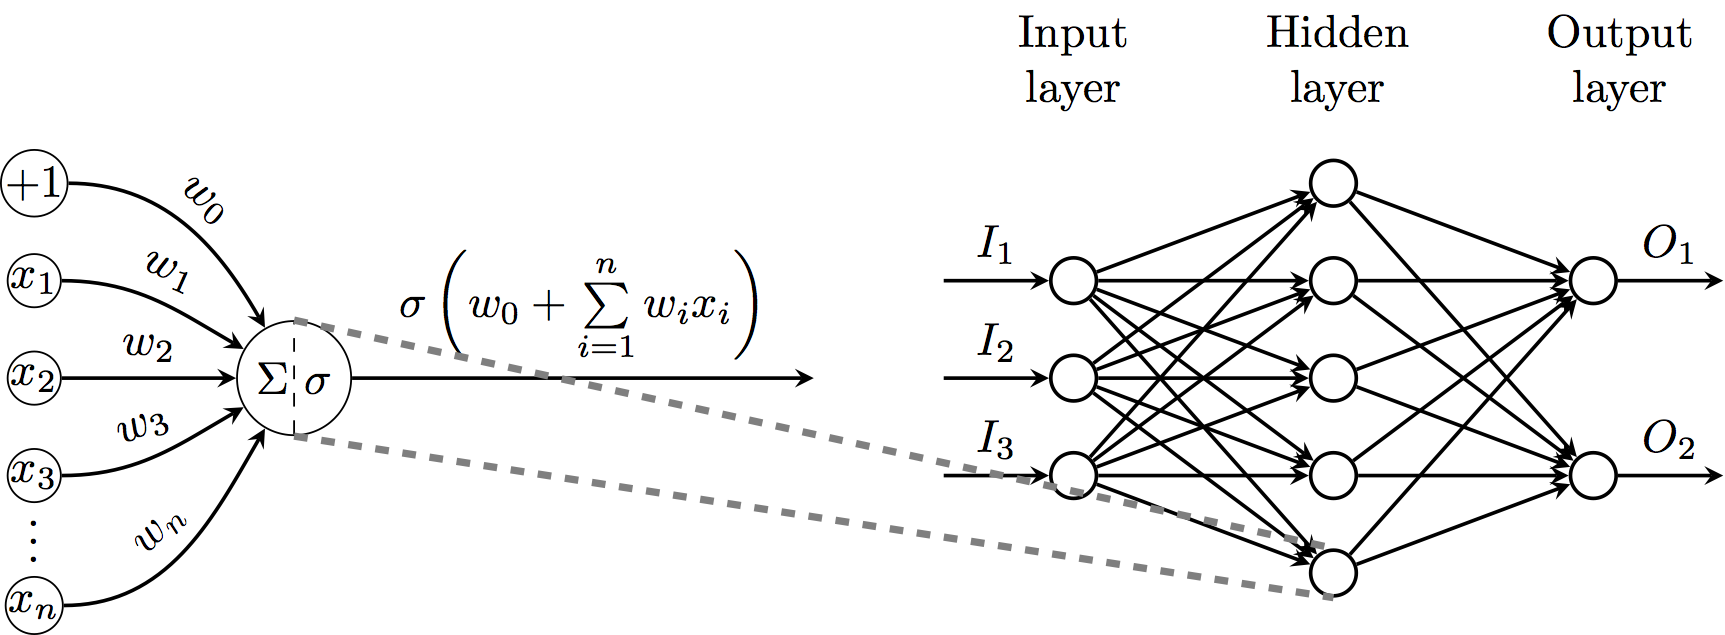
\includegraphics[width=0.95\textwidth]{images/MLP}
	\caption{Multi-Layer-Perceptron (MLP) \cite{Velickovic.2018}}
	\label{fig:mlp}
\end{figure}


Bei diesem Netzwerktyp entspricht der Wert eines Neurons einer linearen Überlagerung $n$ sigmoidaler Funktionen, ausgedrückt durch 

\begin{equation} 
\label{eq:feedforward}
\sigma(w_0 + \sum_{i=1}^{n} w_i x_i)
\end{equation}

Die lineare Überlagerung der Netzwerkgewichte $w_1,w_2,...,w_n$ multipliziert mit den Eingangsgrößen $x_1,x_2,...,x_n$ und verschoben um den Wert $w_0$ wird nochmals durch eine Aktivierungsfunktion transformiert. Mögliche Aktivierungsfunktionen sind die \textit{logistische Sigmoid}-Funktion $\sigma(z) = \frac{1}{1 + e^{-z}}$, die \textit{tangentiale hyperbolische Sigmoid}-Funktion $\phi(z)=\frac{2}{1 + e^{-2z}}-1$ und die \textit{lineare} Funktion $a(z)=z$. \\ 
Die Auswahl der Aktivierungsfunktion ist hierbei vom konkreten Anwendungsfall abhängig. Das Training bzw. die Parametrisierung des Netzes erfolgt nun in zwei Schritten. Im ersten Schritt findet eine Übergabe der Eingangsgrößen $x_1,x_2,...,x_n$ an das Netz statt. Weiterhin nehmen die Netzwerkgewichte $w$ anfangs zufällige Werte an. Da die Eingangsgrößen und die Netzwerkgewichte bekannt sind, kann jeder Neuronenwert nach Gleichung \ref{eq:feedforward} berechnet werden. Die nachfolgenden Neuronenwerte der nächsten Schicht lassen sich somit sukzessive als Funktion der vorherigen Schicht berechnen. Auf diese Weise des Vorwärtsrechnens findet eine Transformation der Eingabegrößen $x_1,x_2,...x_n$ in ein Ausgangssignal $\hat{y}$ statt (in Abbildung \ref{fig:mlp} als $O_1$ und $O_2$ bezeichnet). \\
Der zweite Schritt umfasst nun die Adaptierung der Netzwerkgewichte, sodass die vom Netz herausgegebenen Ausgabegrößen $\hat{y}$ mit den gemessenen Ausgabegrößen $y_i$ möglichst übereinstimmen. Dabei ist es zweckmäßig, die Abweichung zwischen diesen Größen in Form der Fehlerfunktion 

\begin{equation}
E(w) = (y_i-N(x|w))^{2}
\end{equation}

zu beschreiben. Die Adaptierung der Netzwerkgewichte beschränkt sich nun darauf, die Fehlerfunktion zu minimieren. Eine der gängigsten Methoden ist die Methode des Gradientenabstieges. Diese gibt als Adaptionsregel für die Netzwerkgewichte 

\begin{equation}
\label{eq:weight_adapt}
\Delta w_i = \epsilon  (-\nabla E_i) = \epsilon * - \dfrac{\partial E}{\partial w}\bigg|_{w_i}
\end{equation}

mit $\epsilon$ als Lernrate bzw. Adaptionsschrittweite vor. Das Ziel besteht darin, für die Fehlerfunktion $E(w)$ die partiellen Ableitungen $\dfrac{\partial E}{\partial w}\bigg|_{w_i}$ zu identifizieren und gleich null zu setzen. Damit würde die Fehlerfunktion $E(w)$ ein lokales Minima erreichen. Dies geschieht durch die lokale Suche nach dem Minimum der Fehlerfunktion $E(w)$ in Richtung des steilsten Abstiegs. Die Richtung des steilsten Abstiegs entspricht dabei dem negativen Gradienten von $E$ nach den Netzwerkgewichten $w_i$.\\ 
Die Adaption findet für jedes vorhandene Datenpaar $((x_1,x_2,...,x_n)|(y_1))$ statt. Durch das Wiederholen des Adaptionsvorgang passt sich das Netz an das zu modellierende Systemverhalten an. \\

Wie bereits erwähnt, bietet sich die Methode des Gradientenabstieges als ein mögliches Verfahren zur Minimierung der Fehlerfunktion an. Es gibt darüber hinaus in der Literatur eine Vielzahl von Verfahren, die sich nach \cite{Sklyarenko.2002} in folgende Kategorien einteilen lassen:

\begin{itemize}
	\item Gradientenverfahren erster Ordnung
	\item Gradientenverfahren zweiter Ordnung
	\item stochastische Optimierungsverfahren
	\item Verfahren der globalen Optimierung
\end{itemize}


\textbf{Backpropagation-Algorithmus}

Den Verfahren der ersten Kategorie ist gemein, dass die Berechnung des Gradienten des Gütefunktionals

\begin{equation}
\nabla E_i = \dfrac{\partial E}{\partial w}\bigg|_{w_i}
\end{equation}

in jeder Iteration problematisch ist, da sich die Gradienten nicht in einem Schritt berechnen lassen. In der Regel kommt für die Lösung dieses Problems der \textit{Backpropagation}-Algorithmus zum Einsatz. Dieser wendet die Kettenregel an, um die Gradienten in mehrere Faktoren, bestehend aus partiellen Ableitungen, zu zerlegen. Auf diese Weise können die partiellen Ableitungen der letzten Schicht, welche in der Regel bekannt sind, benutzt werden können, um die partiellen Ableitungen der vorangehenden Schichten zu bestimmen. Dies ist gleichbedeutend mit dem Belegen der \textit{Jacobi-Matrix}. \\


\begin{figure} 
	\centering
	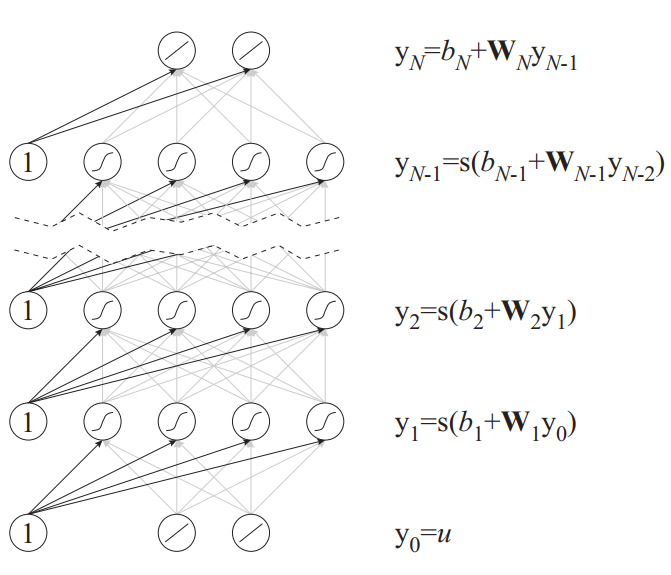
\includegraphics[width=0.65\textwidth]{images/backpropagation2}
	\caption{Multi-Layer-Perceptron \cite{Sturm.2000}}
	\label{fig:backpropagation}
\end{figure}

Die Ermittlung der notwendigen partiellen Ableitungen ergibt sich nach \cite{Sturm.2000} durch folgende Rekursionsformeln \\

\begin{equation}
\begin{aligned}
Y'_{i-1} = Y'_i \cdot S'_i \cdot W_i \\
\dfrac{\partial y_N}{\partial (W_i)_{jk}} = Y'_i \cdot S'_i \cdot \left(\begin{array}{c}
(y_{i-1})_k  \\ ... \\ ... \\ (y_{i-1})_k 
\end{array}\right) \\
\dfrac{\partial y_N}{\partial \vec{b_i}} = Y'_i \cdot S'_i
\end{aligned}
\end{equation}

Dabei enthält die Matrix $Y'_i$ die partiellen Ableitungen der Ausgabegrößen der letzten, also der $N$ten Schicht, nach der $i$ten Schicht. Am Anfang der Rekursion entspricht diese der Einheitsmatrix. Die Matrix $S'_i$ enthält die Ableitungen der Aktivierungsfunktionen der $i$ten Schicht. \cite{Sturm.2000}


Die Ermittlung der partiellen Ableitungen findet also von der letzten bis zur ersten Schicht, also rückwärts, statt. Nach Ermittlung der partiellen Ableitungen aller Schichten, kann die Adaption der Netzwerkgewichte gemäß einer Adaptionsregel, siehe \ref{eq:weight_adapt}, erfolgen. Während des Adaptionsprozesses nimmt der Gesamtfehler ab. Sinkt der Gesamtfehler über alle Netzausgänge $y_1,...,y_m$ unter eine festgelegte Grenze, bricht das Training des Netzes ab. \\


Es bleibt festzuhalten, dass die Anpassungsfähigkeit des Netzes an das nichtlineare Verhalten dynamischer Systeme von folgenden Faktoren abhängt:

\begin{itemize}
	\item Anzahl der Neuronen
	\item Anzahl der Schichten
	\item Wahl des Algorithmus zur Minimierung der Fehlerfunktion
	\item Auswahl der Aktivierungsfunktionen
	\item Initialisierung der Gewichte
	\item Repräsentationsfähigkeit der Trainingsdaten
	
\end{itemize}

Die richtige Auslegung der Parameter für das neuronale Netz stellt eine Herausforderung dar. In Abschnitt \ref{cha:ff_herausforderung} ist eine ausführliche Diskussion über die Auswahl der Netzparameter, vor allem über den Algorithmus und  die Anzahl der Neuronen, enthalten. \\ 

\subsubsection{Herausforderungen bei der Auslegung neuronaler Netze}
\label{cha:ff_herausforderung}

\textbf{Anzahl der Neuronen und Gewichte}

Für die Auslegung neuronaler Netze ist die Abschätzung der Neuronenanzahl relevant. Dabei ist die Festlegung der optimalen Neuronenanzahl eine Abwägung zwischen der Traningszeit, der Generalisierungs- und der Anpassungsfähigkeit an die Nichtlinearitäten des dynamischen Systems. Beispielsweise erhöht nach \cite{Fumumoto.2017} die Anzahl der Neuronen in der verdeckten Schicht die Güte des neuronalen Netzes bei einem Anstieg nichtlinearer Effekte. \\
Nach \cite{.2008} können ebenfalls heuristische Aussagen über eine minimale und maximale Neuronenanzahl getroffen werden. Diese bieten allerdings nur Abschätzungen an. Weiterhin gibt es Vorschläge, die Neuronenanzahl während des Trainings zu adaptieren.\\ 
Dafür lassen sich die Verfahren in zwei Gruppen aufteilen, einmal in konstruktive und reduzierende Verfahren. \\ 
Bei den reduzierenden Verfahren ist die Ausgangsbasis ein bereits trainiertes Netz, welches ein System ausreichend  genau modelliert. \\ 
Nach \cite{Han.682015} sind viele neuronale Netze über-parametrisiert, d.h. sie verfügen über redundante Gewichte. Eine Möglichkeit der Reduktion besteht nun darin, sämtliche Gewichte, deren Wert unter einer vorher definierten Grenze liegt, zu entfernen. Es findet somit eine Unterscheidung zwischen bedeutenden und unbedeutenden Gewichte statt. Nach einer erneuten Trainingsphase findet eine erneute Adaptierung der verbliebenen Netzwerkgewichte statt, sodass diese die erzeugte Abweichung durch das Entfernen der unbedeutenden Gewichte kompensieren können. \cite{Han.682015} \\
Der Einsatz reduzierender Verfahren ist mit Nachteilen verbunden. Zum einen muss ein bereits über-parametrisiertes Netz vorliegen. Die Trainingszeit bei über-parametrisierten Netzen ist in Regel höher also bei nicht über-parametrisierten Netzen. Der Reduktionsvorgang der neuronalen Netze stellt somit einen weiteren Arbeitsschritt dar, dessen zeitlicher Aufwand sich mit dem bereits erhöhten zeitlichen Aufwand für das Training des über-parametrisierten Netzes überlagert. \\
Konstruktive Ansätze dagegen verfolgen den Ansatz, durch Algorithmen ein anfangs mit einer minimalen Topologie ausgestattetes Netz inkrementell mit einer höheren Anzahl an Neuronen und Gewichten auszustatten, wobei jede Modifikation auf ihre Güte untersucht wird. Nach \cite{Parekh.2000} kann dabei durch die Auswahl des Algorithmus erzwungen werden, dass jede weitere Netztopologie einen geringeren Fehler aufweist als die Vorgängertopologie. \\
Der Vorteil bei konstruktiven Ansätzen liegt darin, dass das Entstehen über-parametrisierter Netze von Anfang an unterbunden wird. Über-parametrisierte Netze neigen zum sogenannten \textit{Overfitting}. Beim \textit{Overfitting} sind Netze nicht in der Lage, die Zusammenhänge zwischen Eingangs- und Ausgangsgrößen ausreichend zu verallgemeinern bzw. zu generalisieren. Sie sind zwar in der Lage, den Trainingsdatensatz gut abzubilden, aber nicht in der Lage, für einen unbekannten Datensatz die Ausgangsgröße gut genug zu approximieren. Das gleiche Problem tritt beim \textit{Underfitting} auf. Dabei ist das Netz unter-parametriesiert, d.h. es verfügt nicht über genug Parameter (Netzwerkgewichte), um die Zusammenhänge zwischen Eingags- und Ausgangsgrößen gut genug abzubilden.


\textbf{Trainingsalgorithmen}

Wie in Abschnitt \ref{cha_ff} erwähnt, ist die Methode des Gradientenabstieges eine Möglichkeit der Gewichtsadaption. Jedoch ist diese Methode im Bereich der Gewichtsadaption für neuronale Netze zum größten Teil durch fortschrittlichere Methoden abgelöst worden. Die Limitierungen der Methode des Gradientenabstieges und alternative Algorithmen (z.B. konjugierte Gradienten-Methode, David-Fletcher-Powell-Algorithmus) sind in \cite{WarrenS.Sarle.1994}, \cite{Masters.1995} und \cite{Bishop.2010} sehr gut dokumentiert. Eine weitere Alternative stellt der Levenberg-Marquadt-Algorithmus dar, dessen Implementierung in \cite{Kollias.March1993} diskutiert ist. Weitere Trainingsverfahren sind genetische Algorithmen, deren Einführung in \cite{Hassoun.1996} erörtert worden ist. Diese kommen nicht nur für die Adaptierung der Gewichte, sondern auch für die Adaptierung der Netzwerktopologie (Anzahl der Schichten, Anzahl der Neuronen, Auswahl der Aktivierungsfunktionen, etc.) zum Einsatz, siehe \cite{Bayer.2009} und \cite{StevenA.Harp.1992}.  \\
Weitere Möglichkeiten sind stochastische Methoden des Gradientenabstieges (stochastic gradient descent oder SGD), welche vor allem das Ziel haben, den Trainingsvorgang zu beschleunigen. \cite{JohnDuchi.2010} und \cite{Zeiler.12222012} verändern dafür die Adaptions- bzw. Trainingsrate während der Trainingsphase. Dies führt zu schnelleren bei konvexen, aber zu geringeren Konvergenzgeschwindigkeiten bei nicht-konvexen Fehlerfunktionen. 

Bei der Auswahl von Algorithmen spielt außerdem  die Anzahl der Netzwerkgewichte eine Rolle. Nach \cite{WarrenS.Sarle.1994} eignet sich der Levenberg-Marquardt-Algorithmus bei mehreren Zehnten, der Davidon-Fletscher-Power-Algorithmus bei mehreren Hunderten und der konjugierte Gradienten-Algorithmus bei mehreren Tausenden von Netzwerkgewichten. 


\textbf{Aktivierungsfunktionen} 

Wie in Abschnitt \ref{cha_ff} erwähnt, gibt es für die Auswahl der Aktivierungsfunktion mehrere Möglichkeiten (u.a. die \textit{logistische Sigmoid-}, die \textit{tangentiale hyperbolische Sigmoidfunktion} und die \textit{lineare} Funktion). Während die \textit{lineare} Funktion die Eingangsgröße linear in die Ausgangsgröße transformiert, besteht die Aufgabe der \textit{logistischen Sigmoid-} und der \textit{tangentialen hyperbolischen Sigmoid}- Funktion darin, Nichtlinearitäten in das Netz zu induzieren. So transformiert die \textit{logistische Sigmoid}-Funktion die Eingangsgröße in einen Wertebereich zwischen 0 und 1 und die \textit{tangentiale hyperbolische Sigmoid}-Funktion die Eingangsgröße in einen Wertebereich zwischen -1 und 1. Generell eignet sich jedoch jede differenzierbare Funktion als Aktivierungsfunktion. Die Auswahl der Aktivierungsfunktion der letzten Schicht sollte jedoch auf den Wertebereich der Ausgangsgröße abgestimmt sein. Befindet sich der Wertebereich der Ausgangsgrößen nicht nur in einem Bereich zwischen -1 und 1, kommen dafür in der Regel \textit{lineare} Aktivierungsfunktionen in der letzten Schicht, auch Ausgabeschicht genannt, zum Einsatz. Unterscheidungsmerkmal ist nicht nur der Wertebereich der Ausgangsgröße, sondern auch der Typ der Ausgangsgröße, welcher numerisch, kategorisch oder binär sein kann.  Weiterhin haben die Aktivierungsfunktionen einen Einfluss auf die Konvergenzgeschwindigkeit bzw. Trainingsgeschwindigkeit des Netzes. Nach \cite{Bishop.2010} weisen Netze mit \textit{tangentialen hyperbolischen Sigmoid}-Funktionen höhere Konvergenzzeiten auf als Netze mit \textit{logistischen Sigmoid}-Funktionen. In \cite{Kalman.June1992} dagegen sind die Vorzüge der \textit{tangentialen hyperbolischen Sigmoid}-Funktion gegenüber anderen Aktivierungsfunktionen in Bezug auf mathematischen Eigenschaften während der Trainingsphase diskutiert.

\textbf{Initialisierung der Gewichte}

Wie in Abschnitt \ref{cha_ff} beschrieben, nehmen die Gewichte am Anfang der Trainingsphase zufällige Werte an. Erst im Laufe des Trainings findet die Adaption der Gewichte durch das Minimieren der Fehlerfunktion statt. Dieses findet durch das Anwenden verschiedener Algorithmen (Methode des Gradientenabstieges, Levenberg-Marquardt-Algorithmus etc.) statt. Diese sind allerdings nicht in der Lage, das globale Minimum der Fehlerfunktion zu identifizieren. In der Regel finden die Algorithmen lediglich lokale Minima der Fehlerfunktion. Somit können zwei neuronale Netze, welche mit unterschiedlichen Gewichten initialisiert wurden, aber deren Gewichte mit dem gleichen Algorithmus adaptiert wurden, unterschiedlichen Güten aufweisen, da der Trainingsprozess bei unterschiedlichen lokalen Minima abbricht. In der Literatur finden sich heuristische Ansätze, die initialen Werte für die Gewichte festzulegen. Zum Beispiel wählt \cite{Piovoso.1991b} die initialen Gewichte zwischen der Eingabeschicht und der verdeckten Schicht auf Basis einer Komponentenanalyse und die initialen Gewichte zwischen der verdeckten Schicht und der letzten Schicht auf Basis einer multiplen linearen Regression aus. 

\textbf{Anzahl der Schichten}

Die Netzwerktopologie ist ebenfalls durch die Anzahl der Schichten bestimmt. Nach \cite{Hornik.1989} ist jedoch ein Netz mit nur einer verdeckten Schicht in der Lage, fast jede beliebige Funktion zu approximieren. Die Notwendigkeit einer zweiten Schicht kann sich dann ergeben, wenn stückweise stetige Funktionen zu approximieren sind.


\textbf{Eignung für Regelungsaufgaben}

MLP-Netze gehören zur Gruppe der konnektionistischen Darstellung. Diese sind zwar in der Lage, Funktionen höherer Ordnung abzubilden, allerdings ist eine physikalische Deutung der Parameter in der Regel nicht möglich. Nach \cite{Schroder.2010} sind MLP-Netze nur bedingt für regelungstechnische Aufgaben geeignet, da eine Veränderung der Stützstelle sich global auswirkt und die Gestaltung einer optimalen Netzwerktopologie aufwändig ist.



\textbf{Schlussfolgerung}

Das bisher vorgestellte \textit{MLP-Netz} ist vor allem dazu geeignet, den statischen Zusammenhang zwischen Eingangs- und Ausgangsgrößen abzubilden. \textit{Feedforward-Netze} sind rein vorwärts gerichtete Netze und definieren sich lediglich über die Eingabegrößen und die Parametrisierung der Gewichte. Somit sind \textit{Feedforward-Netze} zustandsfrei. Eine weitere Gruppe statischer Funktionsapproximatoren stellen Netze mit überlagerten Basisfunktionen dar.


\subsection{Netze mit überlagerten Basisfunktionen (statische Funktionsapproximatoren)}

Nach \cite{Schroder.2010} eignen sich vor allem Netze, welche nach der Methode der stützwertbasierten Approximation arbeiten, für regelungstechnische Aufgaben. Diese zeichnen sich vor allem durch kurze Adaptionszeiten und nachweisbare Stabilität aus. Im Gegensatz zu MLP-Netzen, welche zur Gruppe der konnektionistischen Darstellung gehören, verwenden solche Netze lokale Basisfunktionen. Beispiele solcher Basisfunktionen sind die Gaußsche Glockenkurve, Polynome, ein Dreiecksfenster oder die Manhatten-Distanz, siehe Abbildung \ref{fig:basisfunktionen}.

\begin{figure} [H]
	\centering
	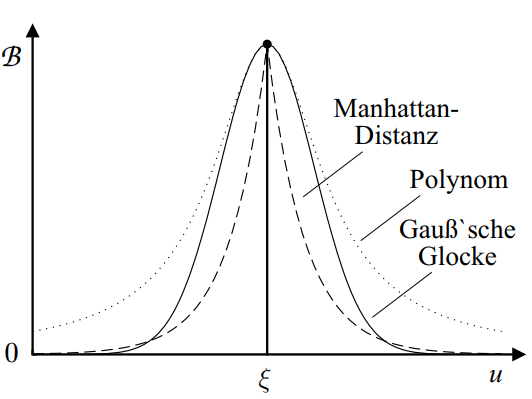
\includegraphics[width=0.65\textwidth]{images/basisfunktionen}
	\caption{Beispiele lokaler Basisfunktionen \cite{Schroder.2010}}
	\label{fig:basisfunktionen}
\end{figure}


Zu den Netzstrukturen mit überlagerten Basisfunktionen gehören das Radial-Basis-Funktion (RBF)-, das General-Regression-Neural-Network (GRNN)-, das harmonisch aktivierte neuronale Netz (HANN) und das Local Linear Model Tree (LOLIMOT)-Netz. \\

In allen vier Netzstrukturen werden die lokalen Basisfunktionen als Aktivierungsfunktionen der Neuronen eingesetzt, siehe beispielsweise das RBF-Netz in Abbildung \ref{fig:rbf}.

\begin{figure} [H]
	\centering
	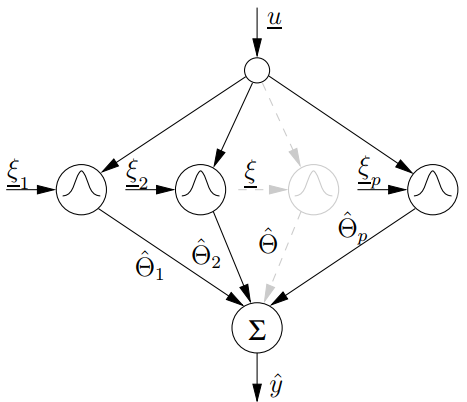
\includegraphics[width=0.65\textwidth]{images/rbf}
	\caption{RBF-Netz mit $p$ Stützstellen  \cite{Schroder.2010}}
	\label{fig:rbf}
\end{figure}


Zudem enthält jede lokale Basisfunktion $\textbf{B}$ einen Vektor \b{$\xi_i$}, welcher die Lage des Zentrums, also das Maximum, der lokalen Basisfunktion angibt. Es findet nun eine Transformation der (mehrdimensionalen) Eingangsgrößen \b{$u$} durch jede Basisfunktion statt, ausgedrückt durch die gesamte Aktivierungsfunktion $\b{\textbf{A}}(\b{u})$

\begin{equation}
\begin{aligned}
\b{\textbf{A}}(\b{u}) = [\textbf{B}(\b{u},\b{$\xi_1$}) \quad \textbf{B}(\b{u},\b{$\xi_2$}) \quad  ... \quad \textbf{B}(\b{u},\b{$\xi_p$})]^{T}
\end{aligned}
\end{equation}

Weiterhin existiert ein gleichlanger Gewichtsvektor \b{$\theta$}, ausgedrückt durch  

\begin{equation}
\begin{aligned}
\b{$\theta$} = [\theta_{1} \quad \theta_2 \quad ... \quad \theta_{p}]^{T}
\end{aligned}
\end{equation}

Am Anfang des Trainings nehmen die Gewichte zufällige Werte an. Die Ausgangsgröße des untrainierten Netzes ergibt sich nun als Skalarprodukt aus dem Aktivierungs- und Gewichtsvektor

\begin{equation}
\begin{aligned}
y(\b{u}) = \b{$\theta$}^T \b{\textbf{A}}(\b{u})
\end{aligned}
\end{equation}

Es wird davon ausgegangen, dass eine trainierte Netzstruktur existiert, deren Approximationsfehler (Differenz zwischen der Ausgangsgröße des Netzes und der zu approximierenden Ausgangsgröße) unter einer beliebig kleinen Schranke liegt. Die Ausgangsgröße $\hat{y}$ eines trainierten Netzes ist durch 


\begin{equation}
\begin{aligned}
\hat{y}(\b{u}) = \hat{\b{$\theta$}}^T \b{\textbf{A}}(\b{u})
\end{aligned}
\end{equation}

beschrieben. Nun kann der Adaptionsfehler zwischen der untrainierten und der trainierten Netzstruktur durch 
\begin{equation}
\begin{aligned}
e(\b{u}) = \hat{y}(\b{u}) - y(\b{u}) = (\hat{\b{$\theta$}}^T -  \b{$\theta$}^T) \; \b{\textbf{A}}(\b{u})
\end{aligned}
\end{equation}

beschrieben werden. Somit kann wie bei den MLP-Netzen die Aufgabe der Adaption bei allen vier Netzstrukturen (RBF-, GRNN-, HANN- und LOLIMOT-Netz) auf die Anpassung der Gewichte reduziert werden. Jede Netzstruktur verwendet jedoch eine unterschiedliche Aktivierungsfunktion, aus der sich für jede Netzstruktur verschiedene Vor- und Nachteile ergeben. \\

Nach \cite{Schroder.2010} weist das RBF-Netz, welches eine Gaußsche Glockenkurve als lokale Basisfunktion verwendet, mangelndes Monotonieverhalten zwischen Stützwerten und mangelndes Extrapolationsverhalten auf. Es kommt z.B. dazu, dass die Ausgangsgröße der Netzstruktur außerhalb des Wertebereiches der Trainingsdaten gegen Null sinkt. Bei regelungstechnischen Anwendungen ist allerdings das Einhalten der Monotonie zwischen Stützwerten und ein nicht gegen null konvergierendes Extrapolationsverhalten erwünscht. \cite{Schroder.2010} \\ 
Diese beiden Nachteile des RBF-Netzes umgeht das GRNN-Netz, da es normierte Gaußsche Glockenkurve als lokale Aktivierungsfunktion verwendet. Durch die Normierung ergeben sich zwei Vorteile gegenüber dem RBF-Netz, erstens wird ein monotoner Verlauf zwischen den Stützwerten sicher gestellt. Der zweite Vorteil besteht darin, dass die Ausgangsgröße des Netzes außerhalb des Wertebereiches der Trainingsdaten den nächstgelegenen Stützwert asymptotisch zustrebt und nicht gegen null geht. Dadurch ergibt sich ein besseres Extrapolationsverhalten für regelungstechnische Anwendungen. Das GRNN-Netz weist jedoch den Nachteil auf, dass für eine hohe Approximationsgenauigkeit eine große Anzahl an Stützstellen und ein somit hoher Rechenaufwand notwendig sind. Insbesondere für die Darstellung periodischer Signale kann dies problematisch sein. \cite{Schroder.2010} \\
Aus diesem Grund kommen für diesen Zweck häufig HANN-Netze zum Einsatz, welche periodische Funktionen als Basisfunktion einsetzen. Nach dem Trainingsvorgang entsprechen die Netzwerkgewichte den Fourierkoeffizienten der reellen frequenzdiskreten Fourierreihe. Durch das Lernergebnis kann somit eine Aussage über die spektrale Zusammensetzung des identifizierten Signals gemacht werden, was für Überwachungs- und Diagnosezwecke interessant ist. HANN-Netze können aber auch erweitert werden, sodass nicht nur periodische, sondern auch nicht-periodische Signale berücksichtigt werden können. \cite{Schroder.2010} \\  
Eine neuere Netzwerkstruktur stellt das \textit{LOLIMOT}-Netz dar, welches eine komplexe, nicht lineare Funktion durch einfachere lokale lineare Modelle mittels Zugehörigkeitsfunktionen überlagert. Ein entscheidendes Unterscheidungsmerkmal zu anderen Netzstrukturen ist, dass nicht nur eine Adaptierung der Gewichte, sondern schrittweise eine Netzstruktur aufgebaut wird. Dabei findet sowohl eine Optimierung in Bezug auf die Anzahl der Neuronen als auch in Bezug auf deren Gültigkeitsbereiches im Eingangsbereich statt. Entscheidende Vorteile des HANN-Netzes sind die schnellere Parameterberechnung und der relativ geringe Anstieg des Parameteranzahl bei steigender Eingangsdimension des Netzes. \cite{Schroder.2010} \\
Sowohl MLP-Netze als auch Netze mit überlagerten Basisfunktionen stellen statische Funktionsapproximatoren auf. Eine weitere Klasse neuronaler Netze sind dynamische Funktionsapproximatoren, deren Grundlagen im nächsten Abschnitt erläutert sind.

\subsection{Rekurrente neuronale Netze (dynamische Funktionsapproximatoren)}

Bei \textit{rekurrenten Netzen} findet - im Gegensatz zu statischen Funktionsapproximatoren - eine Berücksichtigung des zeitlichen Verlaufs der Eingabe- und Ausgabegrößen statt. Dies wird durch den Einsatz von \textit{rekurrenten Kanten} ermöglicht, welche zwei neuronale Netze in aufeinanderfolgenden Zeitschritten miteinander verbinden, siehe Abbildung \ref{fig:recurrent}.  

\begin{figure} [h]
	\centering
	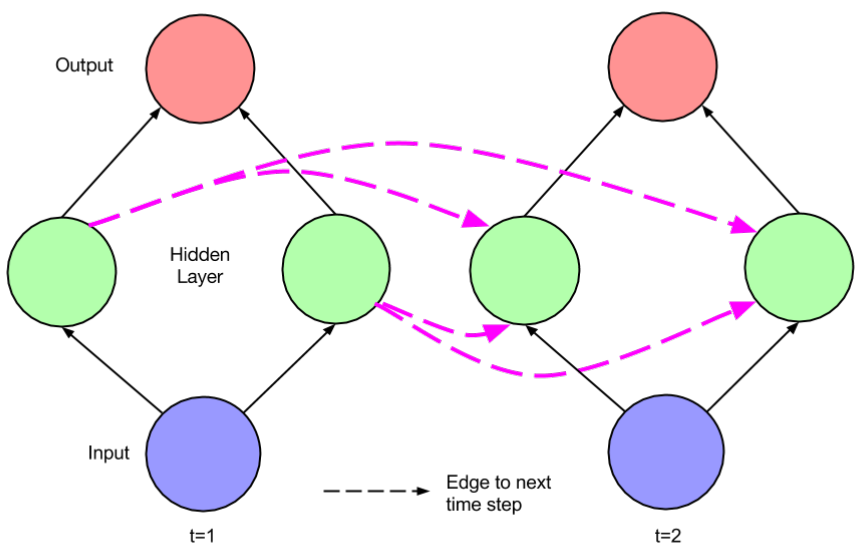
\includegraphics[width=0.65\textwidth]{images/recurrent_net}
	\caption{Rekurrentes Netz \cite{Lipton.5292015}}
	\label{fig:recurrent}
\end{figure}

Die \textit{rekurrenten Kanten} erlauben es, dass die Netzwerkneuronen zum Zeitpunkt $t$ nicht nur die Eingangsgröße $x(t)$, sondern auch die Ausgangsgröße $h^{(t-1)}$ der verdeckten Neuronen des vorherigen Zeitschrittes zum Eingang haben. Der Ausgang des Netzes $\hat{y}^{(t)}$ zum Zeitpunkt $t$ ergibt sich aus dem Ausgang $h^{(t)}$ aller verdeckten Neuronen zum Zeitpunkt $t$. Auf diese Weise beeinflusst die Eingangsgröße $x^{(t-1)}$ zum Zeitpunkt $t-1$ die Ausgangsgröße $\hat{y}^{(t)}$ zum Zeitpunkt $t$. Der Ausgang der verdeckten Neuronen $h^{(t)}$ zum Zeitpunkt $t$ kann nach \cite{Lipton.5292015} durch 

\begin{equation}
h^{(t)} = \sigma(W^{hx}x^{(t)} + W^{hh}h^{(t-1)} + b_h)
\end{equation}

beschrieben werden. Dabei besteht die Matrix $W^{hx}$ aus den konventionellen Gewichten, welche sich zwischen den Eingangsgrößen und den verdeckten Neuronen befinden. Die Matrix $W^{hh}$ dagegen besteht aus \textit{rekurrenten Gewichten}, welche sich zwischen den verdeckten Neuronen des aktuellen und des vorangegangenen Zeitschrittes befinden. Für die Adaptierung der Netzwerkgewichte kommt bei \textit{rekurrenten Netzen} üblicherweise der \textit{Backpropagation-Through-Time(BBTT)}- oder der \textit{Real-Time Recurrent Learning(RTRL)}-Algorithmus zum Einsatz. Der Einsatz dieser Algorithmen ist jedoch mit Problemen verbunden, siehe Abschnitt \ref{cha_recurrent_problem}. \\ 
Im Laufe der Zeit haben sich unterschiedliche Varianten \textit{rekurrenter Netze} entwickelt. Zunächst seien frühere Architekturen \textit{rekurrenter Netze} erläutert.


\subsubsection{Einfache rekurrente Netze (dynamische Funktionsapproximatoren)}
\label{cha:recurrent_simple}
\textbf{Jordan-Netz}

Das \textit{Jordan-Netz} stellt eine der frühen rekurrenten Netzarchitekturen dar, siehe Abbildung \ref{fig:jordan}. 

\begin{figure} [h]
	\centering
	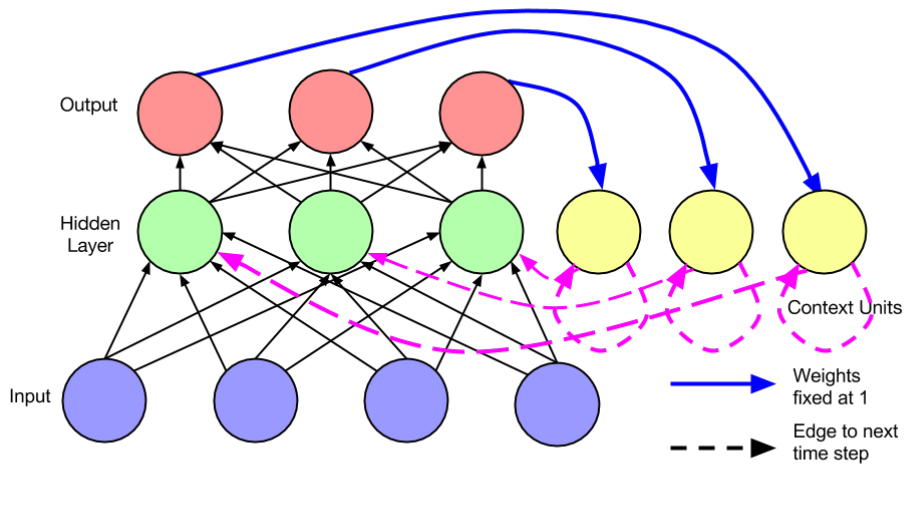
\includegraphics[width=0.65\textwidth]{images/jordan}
	\caption{Jordan-Netz \cite{Lipton.5292015}}
	\label{fig:jordan}
\end{figure}


Das \textit{Jordan}-Netz entspricht einem \textit{Feedforward}-Netz mit einer nachgeschalteten Zustandsschicht, bestehend aus Zustandsneuronen. Diese sind über feste Gewichte (in der Regel haben diese den Wert 1) mit den Neuronen der Ausgangsschicht verbunden. Im nächsten Zeitschritt übergeben diese ihre Ausgangsgröße an die Neuronen der verdeckten Schicht. Durch die festen Gewichte der \textit{rekurrenten} Kanten findet eine Speicherung der Ausgangsgrößen aus dem letzten Zeitschritt in den Zustandsneuronen statt. Auf diese Weise ist das Netz in der Lage Zustände zu speichern, wozu konventionelle \textit{Feedforward-Netze} nicht in der Lage sind. Der Ausgang der verdeckten Schicht $h^{(t)}$ zum Zeitpunkt $t$ ergibt sich nach \cite{Jordan.1997} durch

\begin{equation}
h^{(t)} = \sigma(W^{hx}x^{(t)} + W^{hh}y^{(t-1)} + b^{h})
\end{equation}

Dabei enthält die Matrix $W^{hx}$ die Gewichte zwischen den Eingangsgrößen und den Neuronen in der verdeckten Schicht. Die Matrix $W^{hh}$ dagegen enthält die konstanten Gewichte der \textit{rekurrenten Kanten}. Der Unterschied zu moderneren \textit{rekurrenten Netzen} besteht darin, dass das Jordan-Netz wie ein \textit{Feedforward}-Netz mittels des \textit{Backpropagation}-Algorithmus trainiert wird, wobei die Gewichte der \textit{rekurrenten} Kanten ignoriert bzw. nicht adaptiert werden. Nach \cite{Lipton.5292015} findet - im Gegensatz zu modernen \textit{rekurrenten Netzen} - keine Rückführung des Fehlers über verschiedene Zeitschritte statt. Damit ist dieses Netz nur eingeschränkt für komplexere Dynamiken einsetzbar. \cite{Lipton.5292015} Ein weiterer Nachteil ist, dass die Anzahl der \textit{rekurrenten Kanten} durch die Anzahl der Ausgabeneuronen, also durch die Problemstellung, festgelegt ist. Diesen Nachteil umgeht das \textit{Elman-Netz}.

\textbf{Elman-Netz}

Das \textit{Elman-Netz} stellt ebenfalls eine der früheren \textit{rekurrenten} Netzarchitekturen dar. Der entscheidende Unterschied zum \textit{Jordan-Netz} ist, dass die \textit{rekurrenten Kanten} nicht wie beim \textit{Jordan-Netz} die Ausgabeneuronen mit den Zustandsneuronen, sondern die verdeckten Neuronen mit den Zustandsneuronen verbinden, siehe Abbildung \ref{fig:elman}.

\begin{figure} [h]
	\centering
	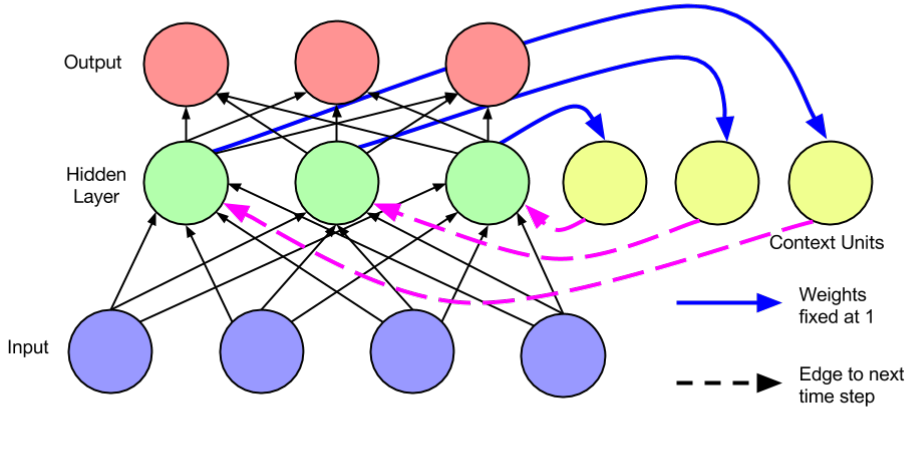
\includegraphics[width=0.65\textwidth]{images/elman}
	\caption{Elman-Netz \cite{Lipton.5292015}}
	\label{fig:elman}
\end{figure}

Das \textit{Elman-Netz} ist wie das \textit{Jordan-Netz} in der Lage, Zustände zu speichern, indem die Zustandsneuronen den Zustand des vorherigen Zeitschrittes im nächsten Zeitschritt an die verdeckten Neuronen übergeben. Somit ergibt sich der Ausgang der verdeckten Schicht $h^{(t)}$ zum Zeitpunkt $t$ nach \cite{Elman.1990} durch 

\begin{equation}
h^{(t)} = \sigma(W^{hx}x^{(t)} + W^{hh}h^{(t-1)} + b^{h})
\end{equation}

Auch hier enthält die Matrix $W^{(hx)}$ die Gewichte zwischen den Eingangsgrößen und den verdeckten Neuronen und die Matrix $W^{(hh)}$ die konstanten Gewichte der \textit{rekurrenten Kanten}.
Wie bei den \textit{Jordan-Netzen} findet das Training des Netzes über den \textit{Backpropagation-Algorithmus} statt, wobei die konstanten Gewichte der \textit{rekurrenten Kanten} ignoriert bzw. nicht adaptiert werden. 
Somit ergibt sich auch beim \textit{Elman-Netz} das Problem, dass keine Rückführung des Fehlers über die Zeit stattfindet, sodass die Anwendbarkeit für komplexere Dynamiken beschränkt ist \cite{Lipton.5292015}. Beim \textit{Elman-Netz} hängt jedoch die Anzahl der \textit{rekurrenten Kanten} nicht von der Anzahl der Ausgabeneuronen, sondern von der Anzahl der verdeckten Neuronen ab. Da die Anzahl der Neuronen in der verdeckten Schicht frei ausgewählt werden kann, hängt die Anzahl der \textit{rekurrenten Kanten} nicht von der Aufgabenstellung ab. Dies ist ein Vorteil gegenüber dem \textit{Jordan-Netz}.

 
\subsubsection{Herausforderungen bei rekurrenten Netzen}
\label{cha_recurrent_problem}

\textbf{Verschwindende und explodierende Gradienten}

\textit{Rekurrente Netze} können - im Gegensatz zu \textit{Feedforward-Netzen} - durch den Einsatz \textit{rekurrenter Kanten} Informationen speichern. Jedoch ist die Anwendung bestimmter Algorithmen für das Netztraining mit Problemen verbunden. \\
Nach \cite{Hochreiter.2001} ist der Einsatz von gradientenbasierten Trainingsalgorithmen, zu denen der \textit{Backpropagation-Through-Time}- und der \textit{Real-Time Recurrent}-Algorithmus gehören, beim Training \textit{rekurrenter Netze} problematisch. Beim  Netztraining können dabei zwei Effekte auftreten. Der erste Effekt umfasst das \textit{Verschwinden der Gradienten}. Dabei nehmen die Gradienten verschwindend kleine Werte an. Dies führt dazu, dass die Adaptierung der Gewichte, also das Training des Netzes, einen sehr hohen Zeitaufwand erfordert oder überhaupt nicht mehr stattfindet. Der zweiter Effekt umfasst das \textit{Explodieren der Gradienten}. Dabei nehmen die Gradienten sehr hohe Werte an, was zu oszillierenden Gewichten und somit zu einer schlechteren Robustheit des Netzes führt. \cite{Hochreiter.2001} \\
\cite{Hochreiter.2001} schlägt vor, das Problem der \textit{verschwindenden Gradienten} durch eine neue Netzstruktur zu lösen. Bei dieser Netzstruktur kommen sogenannte \textit{Long Short-Term Memory}(LSTM)-Zellen zum Einsatz, welche die konventionellen verdeckten Knoten ersetzen, siehe Abschnitt \ref{cha:lstm}.

Die mathematischen Hintergründe und die Charakterisierung der Rahmenbedingungen, welche zu \textit{verschwindenden} oder zu \textit{explodierenden} Gradienten führt, sind in \cite{Pascanu.11212012} erläutert. \cite{Pascanu.11212012} schlägt vor, den Wertebereich der Gewichte durch Regularisierung einzuschränken. Der Einschränkung des Wertebereiches findet derart statt, dass eine zu große Veränderung des Gradienten unterbunden ist. \\


\textbf{Minimierung der Fehlerfunktion}

Wie bei den \textit{Feedforward-Netzen} tritt bei den \textit{rekurrenten Netzen} das Problem auf, dass das Auffinden des globalen Minima der Fehlerfunktion kaum möglich ist. \\
Die Herausforderung besteht darin, durch die Adaption der Gewichte ein möglichst tiefes lokales Minima der Fehlerfunktion zu besetzen. Nach \cite{Dauphin.6102014} sollte bei höher dimensionalen nicht-konvexen Fehlerfunktionen Sattelpunkten eine viel höhere Bedeutung zukommen als lokalen Minima, da die Anzahl der kritischen lokalen Minima bei größeren Netzen exponentiell sinkt. Demnach wird von \cite{Dauphin.6102014} ein Sattelpunkt-freier Newton-Algorithmus vorgeschlagen. Diese Auslegung des Algorithmus unterscheidet sich von der konventionellen Newton-Methode darin, dass die Gewichtsadaptierung derart stattfindet, dass der Wert der Fehlerfunktion sich möglichst weit weg von den kritischeren Sattelpunkten befindet. Es konnten damit zwar Verbesserungen in Hinblick auf die Güte von \textit{rekurrenten Netzen} erzielt werden, allerdings ist für die Anwendung des Sattelpunkt-freien Newton-Methode die rechenintensive Ermittlung der Hesse-Matrix notwendig. \cite{Dauphin.6102014}  

\subsubsection{Moderne rekurrente Netzarchitekturen (dynamische Funktionsapproximatoren)}
\label{cha:lstm}
\textbf{Long Short-Term Memory-Netze}

Wie in \ref{cha_recurrent_problem} erläutern, kann bei \textit{rekurrenten Netzen} der Effekt \textit{verschwindender Gradienten} vorkommen. Zu diesem Zweck führte \cite{Hochreiter.2001} eine neue Netzarchitektur ein, bei dem die verdeckten Neuronen durch sogenannte \textit{Long Short-Term Memory}(LSTM)-Zellen ersetzt sind, siehe Abbildung \ref{fig:lstm}.


\begin{figure} [h]
	\centering
	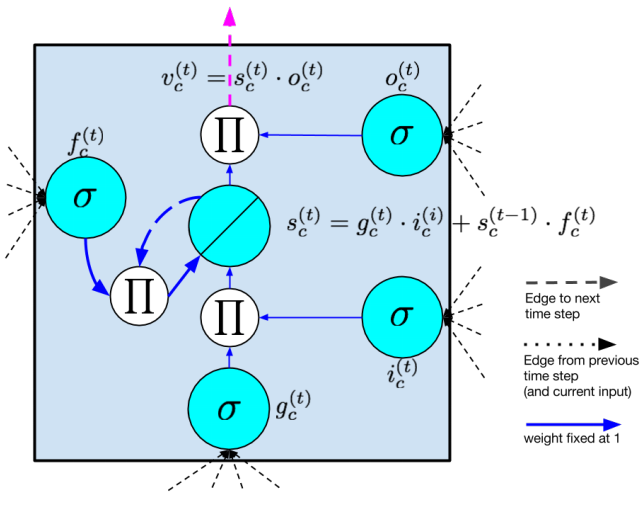
\includegraphics[width=0.65\textwidth]{images/LSTM}
	\caption{Long Short-Termn Memory-Zelle \cite{Lipton.5292015}}
	\label{fig:lstm}
\end{figure}

Nach \cite{Lipton.5292015} bestehen LSTM-Netzarchitekturen aus folgenden Komponenten:

\begin{itemize}
	
	\item Eingangsneuron $g_c^{(t)}$: Das Eingangsneuron transformiert sowohl die Eingangsgrößen $x^{(t)}$ des aktuellen Zeitpunktes $t$ als auch die Ausgänge der verdeckten Schicht $h^{(t-1)}$ aus dem letzten Zeitschritt durch eine Aktivierungsfunktionen. Mögliche Aktivierungsfunktionen sind die $tanh$- und die $sigmoid$-Funktion.  
	\item Eingangsgate $i_c^{(t)}$: Das Eingangsgate enthält eine $sigmoid$-Aktivierungfunktion. Das Gate hat wie das Eingangsneuron die aktuellen Eingangsgrößen $x^{(t)}$ als auch die Ausgänge der verdeckten Schicht $h^{(t-1)}$ aus dem vorherigen Zeitschritt zum Eingang. Die Ausgangsgröße des Gates $i_c{(t)}$ wird nun mit der Ausgangsgröße $g_c^{(t)}$ des Eingagsneurons multipliziert. Damit steuert das Gate den Informationsfluss innerhalb der LSTM-Zelle. Ist die Ausgangsgröße des Gates $i_c^{(t)} = 0$, blockiert das Gate den Informationsfluss. Ist die Ausgangsgröße des Gates $i_c^{(t)}=1$, gibt das Gate den Informationsfluss frei.
	\item Das Zustandsneuron $s_c$ enthält eine lineare Aktivierungsfunktion und soll den internen Zustand der Zelle repräsentieren. Ein Merkmal ist die \textit{rekurrente Kante} mit einem konstanten Gewicht, welche das Zustandsneuron mit sich selbst verbindet. Durch die \textit{rekurrente Kante} können Fehler über mehrere Zeitschritte hinweg in das Zustandsneuron induziert werden. Durch den konstanten Fehlerfluss (in der Literatur oftmals als \textit{contant error carousel} bezeichnet) wird das \textit{Verschwinden} und \textit{Explodieren} der Gradienten unterbunden.
	\item Löschungsgate $f_c$: Durch das Löschungsgate soll das Netz in die Lage versetzt werden, zu lernen, die Inhalte des Zustandsneurons zu löschen. Dies kann vor allem bei kontinuierlich laufenden Netzen hilfreich sein.
	\item Ausgangsgate: Die Ausgangsgröße $v_c^{(t)}$ des Ausgangsgates berechnet sich aus der Multiplikation zwischen der Ausgangsgröße der Zustandsneurons $s_c^{(t)}$ und der Ausgangsgröße des Ausgangsgates $o_c^{(t)}$. In der Regel findet vor der Multiplikation eine Transformation des Zustands $s_c^{(t)}$ durch eine $tanh$-Funktion statt, um den Wertebereich der Ausgangsgrößen festzulegen. \cite{Lipton.5292015}
	
\end{itemize}

Im Gegensatz zu anderen \textit{rekurrenten Netzen} ist es bei \textit{LSTM-Netzen} möglich, den \textit{Backpropagation-Through-Time}-Algorithmus anzuwenden, ohne das es zu einem \textit{Explodieren} oder \textit{Verschwinden der Gradienten} kommt. Dies liegt daran, dass durch die konstante Fehlerrückführung durch die \textit{rekurrente Kante} der Fehler im internen Zustand der \textit{LSTM-Zelle} gespeichert wird.  Auf diese Weise lernen die Gates, wann sie den Fehler blockieren oder durchlassen. \textit{LSTM}-Netze sind vor allem dafür geeignet, langfristige Abhängigkeiten abzubilden. \cite{Lipton.5292015}

\subsubsection{Klassifikation rekurrenter Netze}

Abschließend sei darauf hingewiesen, dass die eben vorgestellten Netze nur einen Bruchteil aller \textit{rekurrenten Netze} darstellen. Nach \cite{Schroder.2010} lassen sich \textit{rekurrente Netze} gemeinhin aufteilen in Netze mit interner und externer Dynamik. Zu den Netzen mit interner Dynamik gehören die \textit{vollrekurrenten} und die partiell \textit{rekurrenten} Netze, wozu die in Abschnitt \ref{cha:recurrent_simple} vorgestellten Jordan- und Elman-Netze gehören. Davon unterscheiden sich sogenannte Netze mit externer Dynamik, wozu das \textit{Time-Delay-Neural Network (TDNN)} in den beiden Variationen \textit{Nonlinear-Output-Error (NOE)} und \textit{Nonlinear-Autoregressiv-with-exogenous-Inputs (NARX)} gehört. Auch die Ansätze basierend auf der Volterra-Funktionalpotentialreihe in der \textit{Nonlinear-Orthogonal-Basis-Functions (NOBF)}- und in der \textit{Nonlinaer-Finite-Impulse-Response (NFIR)}-Form gehören zu den Netzen mit externer Dynamik. \cite{Schroder.2010} 



















   
 
 
 
